\subsection{Amazon DRM (Kiwi)} \label{section:license-amazon}
Amazon started its own application store in October 2010 \cite{amazonBeta} as an alternative go Google Play.
The Amazon appstore opened to the public on the 03/22/2011 \cite{amazonRelease}.
It can be used on Android and \textit{Fire} tablets.
The store comes with its own \gls{drm} since the Google LVL only works with the Google Play Store.
The \gls{drm} is called Kiwi as seen in the reverse engineered code in figure~\ref{fig:amazonFolder}.
\newline
\begin{figure}[h]
    \centering
    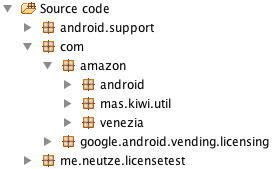
\includegraphics[width=0.3\textwidth]{data/amazonFolder.png}
    \caption{Amazon library structure in decompiled application}
    \label{fig:amazonFolder}
\end{figure}
The prerequisites for using \textit{Kiwi} are similar to the ones of the \gls{lvl}, since the developer requires a developer account on the Amazon Developer Service platform.
According to the description, the library is to \textit{Protect your application from unauthorized use. Without DRM, your app can be used without restrictions by any user.} \cite{amazonDeveloper}
\newline
Amazon has a different approach for implementing the license verification library.
Instead of providing the developer the source code, Amazon injects the mechanism automatically into the application when it is uploaded.
The developer can chose in the developer console whether this should be done or not (see figure~\ref{fig:amazon}).
In order to implement the library, the \gls{apk} is decompiled on the server side, the library is added and the application is compiled again.
This requires the package to be signed with a new signature as described in subsection~\ref{subsection:foundation-android-package}.
Instead of using the developer's own key, Amazon uses a developer specific key.
The information about the key can be retrieved from the developer platform as seen in figure~\ref{fig:amazon}. \cite{amazonDeveloper}
\newline
\begin{figure}[h]
    \centering
    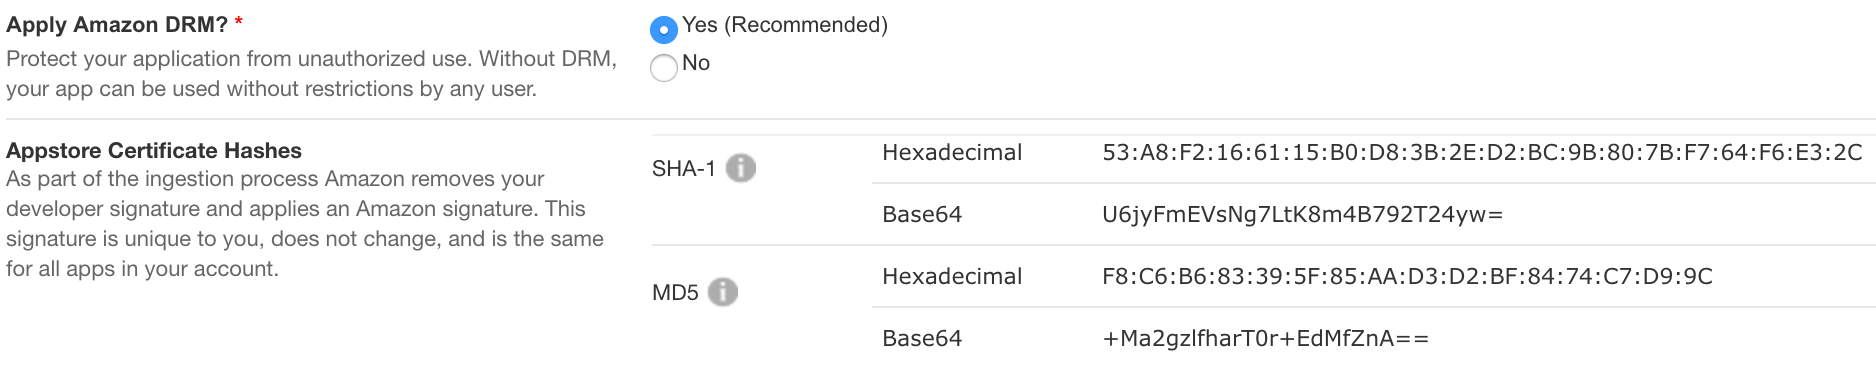
\includegraphics[width=1\textwidth]{data/amazon.png}
    \caption{Developer preferences in the Amazon developer console \cite{amazonDeveloper}}
    \label{fig:amazon}
\end{figure}
The implementation can be analysed with reverse engineering.
The license verification library is wrapped around the original launcher activity of the application.
Its logic is not interweaved with application logic.
The original \textit{onCreate()} method, which is called when the application is started, is renamed to \textit{onCreateMainActivity()} and a new \textit{onCreate()} is injected.
The new method can be seen in code snippet~\ref{codeSnippet:amazonCreate}.
When the application is launched, not only the application is initiated as before, but also the \textit{Kiwi} \gls{drm} functionality is started by calling \textit{Kiwi.onCreate((Activity) this, true)}.
\newline
\lstinputlisting[
  float=h,
  basicstyle=\footnotesize,
  breakatwhitespace=false,
  breaklines=true,
  captionpos=b,
  frame=single,
  numbers=left,
  language=Java,
  linerange={77-80},
  firstnumber=77,
  caption={Amazon's onCreate() injection to call Kiwi license verification as well},
  label={codeSnippet:amazonCreate}
]{data/amazon.java}
The license verification works in combination with Amazon's Appstore application which acts similar to the Google Play Server.
In case Amazon's store is installed on the device, but the user is not signed in, the application prompts the user to sign in.
Since signing in requires an connection to the internet , \textit{Kiwi} indirectly depending on it as well.
It is different when the wrong user is signed in or the store is not even installed.
In this case, the application shows a warning that the app is not owned by the current user, respectively that the Amazon Appstore is required and cannot be found.
